\chapter{교환 대칭성, 스핀, 그리고 두 개의 마이너스 부호}

\section{껍질 채움과 스핀--통계의 문제}

껍질 모형을 살펴보는 일은 전자와 관련된 두 가지 성질에서 시작한다. 전자의 스핀은 1/2이며, 스핀의 두 무차원 투영값은
\begin{equation}
m_s=+\frac12,
\qquad
m_s=-\frac12,
\end{equation}
이다. 또한 전자는 파울리 배타 원리를 따른다. 이 두 사실은 서로 관련되어 있지만, 같은 진술은 아니다.

``같은 상태''라는 표현은 주의해서 써야 한다. 두 전자가 완전한 하나의 입자 상태를 함께 차지할 수는 없다. 그러나 스핀 상태가 다르면 두 전자가 하나의 공간 궤도를 공유할 수 있다. 헬륨을 독립 전자 근사로 다룰 때는 두 전자가 모두 가장 낮은 공간 궤도에 있으며, 하나는 스핀이 위쪽이고 다른 하나는 아래쪽이다. 더 정확히 말하면 ``첫 번째 전자의 스핀은 위쪽이고 두 번째 전자는 아래쪽''인 경우와 ``첫 번째 전자의 스핀은 아래쪽이고 두 번째 전자는 위쪽''인 경우는 얽힌 두 전자 스핀 상태에 속한다.

이것은 오래된 껍질 모형 근사일 뿐이다. 이 근사는 전자 사이의 상호작용을 무시하며, 간단한 셈을 위해 사용한다. 리튬에서는 처음 두 전자가 가장 낮은 공간 궤도를 반대 스핀으로 채운다. 세 번째 전자는 이 두 완전한 상태 중 어느 쪽에도 들어갈 수 없으므로 더 높은 궤도를 차지해야 한다.

다음 단계는 익숙한 궤도 각운동량 도표를 살펴보는 것이다. 다음 값을 갖는 부분공간을
\begin{equation}
\ell=0,\qquad \ell=1,\qquad \ell=2
\end{equation}
각각 \(S\), \(P\), \(D\) 상태라고 부른다. \(\ell\)의 고정된 값에는 궤도 상태가
\begin{equation}
2\ell+1
\end{equation}
개 있으므로,
\begin{equation}
\ell=0\Rightarrow 1,
\qquad
\ell=1\Rightarrow 3,
\qquad
\ell=2\Rightarrow 5.
\end{equation}
쿨롱 문제에는 추가 축퇴가 있다. 서로 다른 \(\ell\) 부분공간에 속하는 방사형 준위들이 같은 에너지를 가질 수 있다. 껍질 채움 논의에서 다음 껍질에는 \(S\) 궤도 하나와 \(P\) 궤도 세 개가 있다. 따라서 공간 상태는
\begin{equation}
1+3=4
\end{equation}
개이다. 스핀을 고려하면 그 수가 두 배가 된다:
\begin{equation}
2(1+3)=8.
\end{equation}

리튬부터 네온까지 단순한 순서로 이 완전한 전자 상태 여덟 개가 채워진다. 닫힌 껍질을 지나면 나트륨에는 다시 바깥 전자가 하나 남는데, 이것이 이 거친 모형에서 나트륨이 리튬과 비슷하게 보이는 이유다. 여기서 목표는 화학이 아니다. 중요한 점은 반정수 스핀과 배타 원리가 함께 나타난다는 것이다.

광자는 대조적인 사례다. 광자의 스핀은 정수이며, 광자는 배타 규칙을 따르지 않는다. 고전 전자기파는 동일한 모드를 차지하는 많은 광자에 해당한다. 보손은 하나의 상태에 모일 수 있지만, 동일한 페르미온은 완전한 하나의 상태를 두 번 이상 차지할 수 없다. 그렇다면 이 두 짝이 서로 바뀔 수도 있었을까? 즉, 배타 원리가 없는 반정수 스핀이나 배타 원리가 있는 정수 스핀이 가능했을까? 공간 차원이 3인 경우 스핀--통계 관계에 따르면 그렇지 않다. 익숙한 진술은 공간 차원이 1 또는 2일 때는 단서를 달아야 하며, 여기서는 장 이론 결과의 증명을 다루지 않는다.

\begin{classroomqa}
\lecturetimestamp{00:11:48}
\audiencequestion{하나의 상태를 차지할 수 있는 보손 양자 수에 상한이 있나요?}
\lecturerresponse{아니요. 보손은 점유 수에 제한이 없으며, 같은 상태에 모이는 경향이 있습니다.}
\end{classroomqa}

\section{다입자 파동함수}

이 연결 관계를 교환에서 생기는 마이너스 부호와 회전에서 생기는 마이너스 부호, 두 가지를 통해 살펴보겠다. 먼저 교환을 다루고, 일단 스핀은 생략하자.

\(x_i\)를 입자 \(i\)의 위치라고 하자. 아래 첨자는 입자 표기이지 데카르트 성분이 아니다. 세 공간 좌표는 하나의 기호 \(x_i\)로 줄여 썼다. \(n\)개 입자의 위치 기저는
\begin{equation}
\lvert x_1,x_2,\ldots,x_n\rangle.
\end{equation}
이다. 추상 상태 \(\lvert\Psi\rangle\)에 대해 좌표 파동함수는
\begin{equation}
\psi(x_1,x_2,\ldots,x_n)
=
\langle x_1,x_2,\ldots,x_n\mid\Psi\rangle.
\end{equation}
이다. 그 절댓값의 제곱,
\begin{equation}
\bigl\lvert\psi(x_1,x_2,\ldots,x_n)\bigr\rvert^2,
\end{equation}
은 입자 \(1\)가 \(x_1\)에, 입자 \(2\)가 \(x_2\)에 있는 등의 경우에 대한 결합 확률 밀도다.

이제 입자들이 동일하다고 하자. 먼저 한 전자는 파란색으로, 다른 전자는 빨간색으로 칠했다고 상상해 보자. 그러면 ``파란색 전자가 \(x_1\)에 있고 빨간색 전자가 \(x_2\)''인 경우는 ``파란색 전자가 \(x_2\)에 있고 빨간색 전자가 \(x_1\)인 경우와 구별될 수 있다''. 실제 전자에는 그런 색깔이나 개별 표지가 없다. 장부상 표지를 서로 바꾸어도 새로운 물리적 배열이 생기지는 않는다.

전체 위상은 확률이나 기댓값을 바꾸지 않는다. 따라서 교환 고유 상태에 있는 상태의 좌표 파동함수는
\begin{equation}
\psi(x_2,x_1)=\eta\,\psi(x_1,x_2),
\qquad
\lvert\eta\rvert=1.
\end{equation}
를 만족할 수 있다. 같은 교환을 두 번 적용하면 원래 인수 순서로 돌아오며,
\begin{equation}
\eta^2=1,
\end{equation}
가 되므로 가능한 교환 고윳값은 두 가지다:
\begin{equation}
\eta=+1
\qquad\hbox{or}\qquad
\eta=-1.
\end{equation}

\editorialnote{교환을 두 번 수행하는 대수적 관계는 상태가 교환에 대해 확정된 성질을 갖는다고 놓은 뒤에야 가능한 고윳값을 결정한다. 같은 종에 속하는 허용 상태가 하나의 교환 부문에만 속한다는 추가 제약은 물리적 규칙이며, \(\eta^2=1\)만으로 따라 나오지는 않는다. 아래의 배타 원리 논증에도 같은 단서가 적용된다. 페르미온 부문을 선택하면 반대칭성이 배타를 뜻하지만, 교환 대수만으로 그 부문이 선택되는 것은 아니다.}

보손의 허용 파동함수는 대칭이고,
\begin{equation}
\psi_B(x_1,x_2)=\psi_B(x_2,x_1),
\end{equation}
페르미온의 허용 파동함수는 반대칭이다:
\begin{equation}
\psi_F(x_1,x_2)=-\psi_F(x_2,x_1).
\end{equation}
마이너스 부호가 상태 전체에 곱해지면 관측할 수 없지만, 진폭을 더할 때는 중요하다. 교환 대칭성이 관측 가능한 결과를 낳는 방식이 바로 이것이다.

\section{곱, 합, 그리고 배타 원리}

먼저 두 입자를 같은 한 입자 궤도 \(\psi_0\)에 배정해 보자. 두 파동함수의 곱은
\begin{equation}
\psi_0(x_1)\psi_0(x_2).
\end{equation}
이다. 입자 좌표를 교환하면
\begin{equation}
\psi_0(x_2)\psi_0(x_1)
=
\psi_0(x_1)\psi_0(x_2).
\end{equation}
이 된다. 파동함수의 값은 연산자가 아니라 수이므로 인수들은 교환 가능하다. 같은 상태의 곱은 대칭이다. 이는 허용되는 보손 상태의 형태지만, 동일한 두 페르미온을 기술할 수는 없다.

이제 입자들을 서로 다른 한 입자 궤도에 배정하자:
\begin{equation}
\psi_0(x_1)\psi_1(x_2).
\end{equation}
교환하면
\begin{equation}
\psi_0(x_2)\psi_1(x_1).
\end{equation}
이 된다. 서로 다른 함수에 대해서는 교환된 곱이 일반적으로 원래 식과 같지도, 그 음수와 같지도 않다. 따라서 단순한 곱은 요구되는 어느 교환 대칭성도 갖지 않는다. 그렇다고 한 입자가 \(\psi_0\)를 차지하고 다른 입자가 \(\psi_1\)를 차지하는 것이 금지되는 것은 아니다. 두 입자 상태가 두 배정을 결합한 형태여야 한다는 뜻이다.

대칭 조합은
\begin{equation}
\psi_B^{(01)}(x_1,x_2)
\propto
\psi_0(x_1)\psi_1(x_2)
+
\psi_0(x_2)\psi_1(x_1),
\end{equation}
이고, 반대칭 조합은
\begin{equation}
\psi_F^{(01)}(x_1,x_2)
\propto
\psi_0(x_1)\psi_1(x_2)
-
\psi_0(x_2)\psi_1(x_1).
\end{equation}
이다. 교환 논증에는 정규화가 필요 없으므로 비례 기호로 충분하다. 두 상태 모두 각 궤도에 입자 하나씩을 포함하며, 구별할 수 없는 두 배정을 결합하는 방식만 다르다.

이제 궤도함수들이 일치한다고 하자. 보손 조합은 다음과 같이 된다.
\begin{align}
\psi_B^{(00)}(x_1,x_2)
&\propto
\psi_0(x_1)\psi_0(x_2)
+
\psi_0(x_2)\psi_0(x_1)\\
&=
2\psi_0(x_1)\psi_0(x_2),
\end{align}
이는 영이 아니다. 페르미온 조합은 다음과 같다.
\begin{align}
\psi_F^{(00)}(x_1,x_2)
&\propto
\psi_0(x_1)\psi_0(x_2)
-
\psi_0(x_2)\psi_0(x_1)\\
&=0.
\end{align}
반대칭 교환 규칙을 적용하면 배타 원리가 따른다. 두 페르미온이 같은 단일 입자 상태에 있는 반대칭 상태는 영이 아닌 상태일 수 없다.

다입자 상태에서는 두 인수를 맞바꾸는 임의의 교환에 이 규칙이 적용된다. 교환을 하면 보손 파동함수는 변하지 않고 페르미온 파동함수는 부호가 바뀐다. 같은 교환을 반복하면 두 경우 모두 항등 변환이 된다. 놀라운 점은 한 번의 교환이 관측 가능한 입자 표지를 바꾸지는 않으면서 페르미온 상태의 부호를 바꾼다는 것이다.

\section{완전한 입자 표지에 포함되는 스핀}

이제 약간만 바꾸어 스핀을 다시 포함하자. 한 입자 진폭은 위치와 이산적인 스핀 표지 모두에 의존한다:
\begin{equation}
\psi(x,\sigma),
\end{equation}
여기서 \(\sigma=+1\) 또는 \(-1\)는 선택한 \(\sigma_z\) 결과를 나타낸다. 절댓값의 제곱은 주어진 위치와 스핀 표지에 대한 결합 확률 밀도다.

다입자 파동함수는
\begin{equation}
\psi(x_1,\sigma_1;\,x_2,\sigma_2;\,\ldots).
\end{equation}
이다. 교환은 위치만이 아니라 두 입자에 속한 모든 것을 맞바꾼다:
\begin{align}
\psi_B(x_1,\sigma_1;\,x_2,\sigma_2)
&=
+\psi_B(x_2,\sigma_2;\,x_1,\sigma_1),\\
\psi_F(x_1,\sigma_1;\,x_2,\sigma_2)
&=
-\psi_F(x_2,\sigma_2;\,x_1,\sigma_1).
\end{align}
이것이 서두의 껍질 모형 진술을 정확히 표현한 것이다. 두 전자는 스핀을 포함한 완전한 상태가 서로 다를 때만 하나의 공간 궤도를 공유할 수 있다.

\begin{classroomqa}
\lecturetimestamp{00:34:33}
\audiencequestion{교환 대칭성은 순열군의 한 사례인가요?}
\lecturerresponse{그렇습니다. 입자 교환은 순열이며, 플러스 또는 마이너스 변환 법칙은 순열군의 표현을 이룹니다.}
\end{classroomqa}

\begin{classroomqa}
\lecturetimestamp{00:35:12}
\audiencequestion{두 입자 상태를 구성할 때 한 입자 파동함수의 합이 아니라 곱을 쓰는 이유는 무엇인가요?}
\lecturerresponse{합은 한 입자가 중첩 상태에 있음을 나타냅니다. 곱은 두 입자 텐서곱 공간에 속하며, 입자 하나씩을 각 한 입자 상태에 배정했음을 나타냅니다.}
\end{classroomqa}

완전한 표지의 교환을 아래 판서에 나타냈다.\footnote{--스핀 표지의 순서는 판독 가능한 판서 화면과 00:33:43부터 00:34:25까지의 주변 설명을 바탕으로 복원했다.}
\begin{figure}[htbp]
\centering
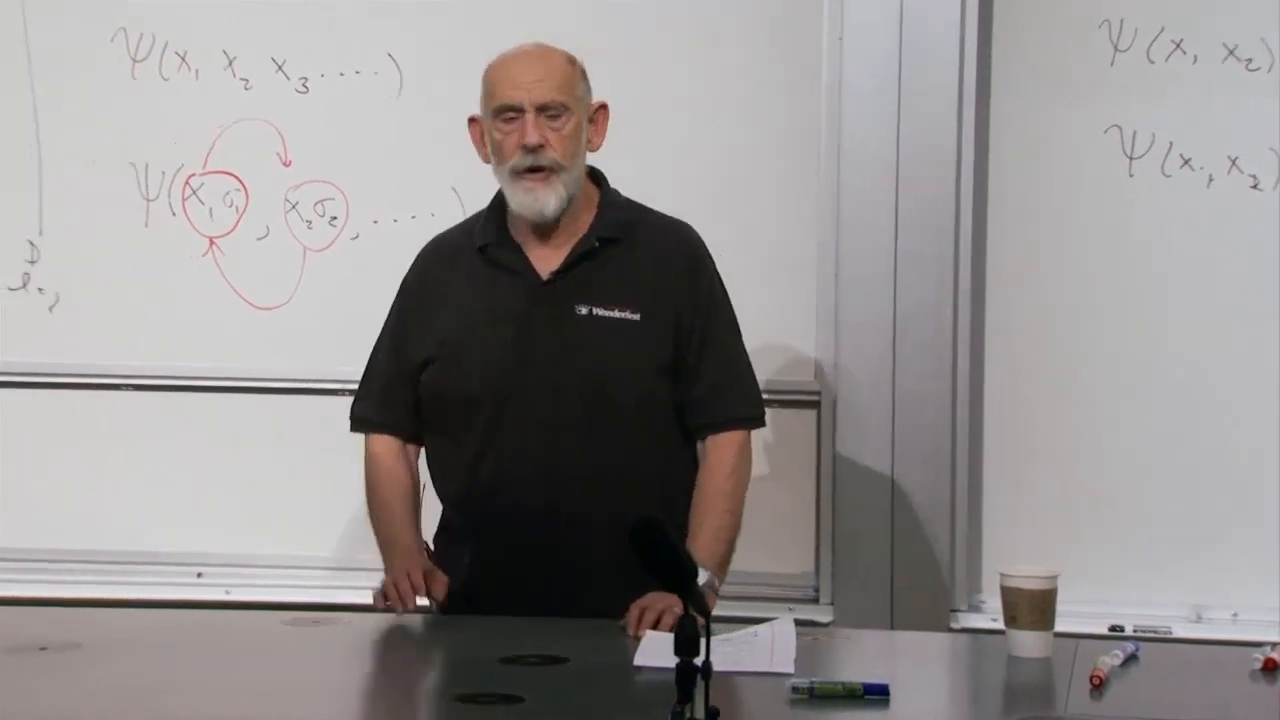
\includegraphics[width=0.9\linewidth]{lecture_05_frame_03.png}
\caption{동일한 두 입자를 교환하면 위치--스핀 표지 전체가 맞바뀐다. 보손 상태는 변하지 않지만 페르미온 상태는 부호가 바뀐다.}
\lectureframe{00:35:25}
\end{figure}

여기에는 선형성의 서로 다른 두 가지 쓰임이 있다. 한 입자의 경우,
\begin{equation}
\alpha\psi_0(x)+\beta\psi_1(x)
\end{equation}
는 두 가능성의 중첩이다. 두 입자의 경우,
\begin{equation}
\psi_0(x_1)\psi_1(x_2)
\end{equation}
는 두 입자 좌표를 갖는 공간 위의 곱 진폭이다. 대칭화 또는 반대칭화는 이 곱에 교환된 항을 결합한다.

\begin{classroomqa}
\lecturetimestamp{00:36:13}
\audiencequestion{입자 교환으로 간섭 효과가 생기나요?}
\lecturerresponse{그렇습니다. 같은 상태에서 페르미온 진폭이 사라지는 현상은 교환된 두 기여가 상쇄 간섭을 일으키는 것으로 이해할 수 있습니다.}
\end{classroomqa}

\begin{classroomqa}
\lecturetimestamp{00:37:13}
\audiencequestion{파울리도 이와 같은 대칭성 논증으로 배타 원리를 도출했나요?}
\lecturerresponse{파울리는 경험적 사실에서 출발해 그 사실을 표현할 수 있는 수학적 틀을 찾았습니다. 처음부터 더 근본적인 이론으로 배타 원리를 도출한 것은 아닙니다.}
\end{classroomqa}

반대칭성은 경험적 배타 규칙을 표현하는 수학적 틀을 제공한다.

\begin{classroomqa}
\lecturetimestamp{00:39:01}
\audiencequestion{입자 교환 간섭은 가능한 경로들 사이의 간섭과 관련이 있나요?}
\lecturerresponse{그렇습니다. 한 경우에는 두 입자가 서로 교차하지 않고 지나가고, 다른 경우에는 교차하여 서로 바뀐 목적지로 간다. 보손의 경우 진폭이 더해지고, 페르미온의 경우 상쇄될 수 있습니다.}
\end{classroomqa}

교환에서 첫 번째 마이너스 부호가 나온다. 두 번째는 회전에서 나온다.

\section{두 번째 마이너스 부호: \texorpdfstring{\(2\pi\)}{2 pi}}

완전한 회전은 아무 일도 일으키지 않는 것처럼 보인다. 보통의 기하학적 방향은 모두 각도 \(2\pi\)만큼 회전한 뒤 출발점으로 돌아온다. 그러나 돌아와야 하는 것은 확률과 기댓값이다. 교환의 경우와 마찬가지로 상태 벡터 자체는 전체 위상만큼 달라진 채 돌아올 수 있다.

\begin{classroomqa}
\lecturetimestamp{00:42:12}
\audiencequestion{회전축은 어느 축으로 택하며, 생성자는 궤도 각운동량, 스핀, 아니면 둘 다인가요?}
\lecturerresponse{외부 축을 하나 택하면 되며, 아래에서는 \(z\)축으로 하겠습니다. 생성자는 궤도와 스핀 기여를 모두 포함하는 총 각운동량입니다. 스핀 자체가 선택한 축을 향할 필요는 없습니다.}
\end{classroomqa}

\editorialnote{이 논의의 각운동량 공식에서는 \(\hbar=1\)로 놓으므로, \(m\)는 \(J_z\)의 무차원 고윳값이다.}

\(\psi(\theta)\)를 회전 매개변수가 각도 \(\theta\)만큼 변할 때 얻는 상태라고 하자. 여기서 사용하는 규약에서는
\begin{equation}
J_z\psi(\theta)
=
-i\frac{\partial}{\partial\theta}\psi(\theta).
\end{equation}
이다. \(J_z\)가 정해진 상태에 대해서는
\begin{equation}
J_z\psi(\theta)=m\psi(\theta).
\end{equation}
이다. 두 식을 결합하면
\begin{equation}
-i\frac{\partial}{\partial\theta}\psi(\theta)
=
m\psi(\theta),
\end{equation}
을 얻으며, 그 해는
\begin{equation}
\psi(\theta)=e^{im\theta}\psi(0).
\end{equation}
이다.

\(m\)의 허용값은 정수 또는 반정수다. 따라서
\begin{equation}
\psi(2\pi)
=
\begin{cases}
+\psi(0), & m\in\mathbb Z,\\[4pt]
-\psi(0), & m\in\mathbb Z+\tfrac12.
\end{cases}
\end{equation}
이다. 한 바퀴 더 회전하면 두 경우 모두
\begin{equation}
\psi(4\pi)=\psi(0)
\end{equation}
가 된다. 이것이 두 번째 마이너스 부호다. 반정수 각운동량 다중항에 속하는 상태는 \(2\pi\) 회전할 때 부호가 바뀐다.

부호는 \(\lvert\psi\rvert^2\)를 바꾸지 않으므로 상태 전체에 곱해져 있을 때는 관측되지 않는다. 그래도 반정수 스핀 상태에 대한 \(2\pi\) 회전은 항등 변환으로 나타나지 않는다. 이 부호를 다른 결맞은 진폭에 대한 상대적인 부호로 만들면 차이를 관측할 수 있다.

\section{\texorpdfstring{\(2\pi\) 및 \(4\pi\)}{2파이 및 4파이 회전 경로}}

\(2\pi\)와 \(4\pi\)의 차이는 추가 대수 전개 없이도 드러낼 수 있다. 한 손으로 컵을 잡고 놓지 않은 채 한 바퀴 돌려 보자. 컵은 원래 방향으로 돌아오지만 팔은 꼬인다. 한 바퀴 더 돌리면 컵의 회전 방향을 거꾸로 하지 않고도 팔을 원래 위치로 되돌릴 수 있다.

이와 관련된 구성에서는 구를 상자 안에 두고 끈으로 구와 상자를 연결한다. 구를 \(2\pi\)만큼 돌리면 끈이 엉킨다. 보통의 3차원 공간에서는 \(4\pi\) 회전에 해당하는 엉킴을 풀 수 있다. 중요한 것은 구의 최종 방향만이 아니라 회전 공간을 통과하는 경로다.

\begin{classroomqa}
\lecturetimestamp{00:54:22}
\audiencequestion{구를 같은 축을 중심으로 두 번 돌리면 끈을 정말 풀 수 있나요? 그러려면 또 다른 공간 차원이 필요한가요?}
\lecturerresponse{\(4\pi\) 경로는 보통의 3차원 공간에서 풀 수 있습니다. 시간은 운동을 매개변수화할 뿐, 또 다른 공간 방향이 아닙니다. \(2\pi\) 경로는 이런 방식으로 풀 수 없지만, \(4\pi\) 경로는 풀 수 있습니다.}
\end{classroomqa}

이 시연은 회전군의 형식 이론을 전개하지 않고도 풀리지 않는 \(2\pi\) 경로와 풀 수 있는 \(4\pi\) 경로의 차이를 보여준다.

\section{벨트 그림에서의 교환과 회전}

이제 두 마이너스 부호를 나란히 살펴보자. 동일한 두 페르미온을 교환하면 결합 파동함수의 부호가 바뀐다. 반정수 스핀 상태를 \(2\pi\)만큼 회전해도 부호가 바뀐다. 벨트를 이용하면 두 작용 사이의 기하학적 관계를 볼 수 있다.

벨트의 아래쪽 끝 두 개가 서로 바뀌도록 벨트를 놓는다. 다른 관점에서 보면 같은 벨트에 \(2\pi\) 꼬임이 있다. 교환과 \(2\pi\) 회전을 함께 수행하면 꼬임이 사라지고 꼬이지 않은 벨트가 남는다. 이 결합 과정은 연속적으로 아무것도 하지 않는 상태로 줄일 수 있다.\footnote{강의에서는 교환--회전 관찰을 David Finkelstein에게 귀속한다. 원자료 기록에는 특정 출판물이 제시되어 있지 않으므로, 여기서는 그 이름을 해당 귀속의 형태로만 유지한다.}

\begin{classroomqa}
\lecturetimestamp{01:01:12}
\audiencequestion{이것은 입자의 위상에 관한 설명이 아니라 단지 벨트가 공간에 놓이는 방식에 관한 설명인가요?}
\lecturerresponse{벨트를 시공간에서의 입자 이력으로 해석할 수 있습니다. 시간이 위쪽으로 흐르게 놓으면 벨트를 가로지르는 단면에 입자와 같은 물체가 나타납니다. 쌍이 생성되고, 한 물체가 \(2\pi\)만큼 회전하며, 동일한 두 물체가 교환됩니다. 이 이력에서는 회전 위상과 교환 위상이 상쇄됩니다.}
\end{classroomqa}

이 이력에서는 위상을 어떻게 셈하는지 분명하게 드러난다. 입자가 없는 상태에서 시작한다. 서로 떨어진 두 곳에서 입자--반입자 쌍을 생성하여 중간 시점에 입자 네 개를 만든다. 한 입자를 \(2\pi\)만큼 회전시키는 동안 구성의 다른 곳에서는 동일한 두 입자를 교환한다. 이 전체 이력은 쌍을 생성한 뒤 다시 소멸시키는 기본 이력으로 변형할 수 있다. 여기서 다루는 부호 셈에서 이 자명한 이력에는 추가 위상이 없다. \(\eta_{\mathrm{rot}}\)와 \(\eta_{\mathrm{ex}}\)를 두 부호라고 하면, 말로 설명한 상쇄는 다음과 같이 간단히 쓸 수 있다.\footnote{이 위상 방정식은 01:06:50부터 01:07:18까지 설명된 상쇄를 기록한 것이다. 강의에서는 이 구성을 엄밀한 증명이 아니라 시사적인 논증으로 제시한다.}
\begin{equation}
\eta_{\mathrm{rot}}\eta_{\mathrm{ex}}=1.
\end{equation}

\begin{classroomqa}
\lecturetimestamp{01:03:34}
\audiencequestion{두 입자가 각각 \(\pi\)만큼 움직인 뒤 방향을 다시 잡게 하면 교환을 회전과 관련지을 수 있나요?}
\lecturerresponse{그 구성은 관련된 수학을 반영할 수 있지만, 서로 별개인 \(\pi\) 회전을 두 번 사용합니다. 여기서 분석하는 과정에는 \(2\pi\) 회전이 한 번 포함되므로 두 논증은 동일하지 않습니다.}
\end{classroomqa}

이 논증은 입자와 같은 물체를 생성하고 소멸할 수 있다는 가능성에 의존한다. 입자가 영원히 존재하는 이론이라면 이런 형태의 논증은 성립하지 않는다. 또한 이 논증을 스핀--통계 정리의 표준 증명으로 제시하는 것도 아니다. 여기서 보이려는 것은 교환 부호와 회전 부호가 서로 들어맞는 위상학적 이유다.

\section{덩어리, 거울상, 그리고 소멸}

이 구성은 국소화된 장 구성으로도 반복할 수 있다. 하나 이상의 장이 거의 모든 곳에서 진공값을 취하지만 작은 영역에서는 영이 아닌 모양과 구조를 갖는다고 하자. 이렇게 국소화된 구성을 덩어리(lump)라고 한다.

이제 첫 번째 배치의 적절한 거울상으로 두 번째 배치를 만든다. 하나를 입자, 다른 하나를 반입자라고 하자. 두 배치를 서로 가까이 가져간다. 장 배치에서 대응하는 부분들이 만나 서로를 지운다. 중간 단계에서는 덩어리의 일부가 이미 사라졌지만 다른 부분은 남아 있을 수 있다. 변형을 계속하면 남은 구조도 사라져 장이 진공 배치로 돌아간다. 벨트에서 서로 반대 방향으로 놓인 비틀림 두 개도 같은 모습을 보여준다. 두 비틀림을 밀어 붙이면 풀린다.

이 과정은 거꾸로도 진행할 수 있다. 빈 공간에서 덩어리와 그 거울상 짝이 생길 수 있다. 이런 쌍 두 개를 생성하고, 덩어리 하나를 \(2\pi\)만큼 회전시키고, 동일한 두 덩어리를 교환한 다음, 쌍을 다시 소멸시킬 수 있다. 그러면 같은 교환--회전 상쇄가 적용된다. 이는 여전히 이 구성의 직관적 확장이며, 모든 국소화된 들뜸에 대한 정리는 아니다.

\begin{classroomqa}
\lecturetimestamp{01:11:30}
\audiencequestion{이러한 덩어리형 장 배치가 물리적으로 실현되나요?}
\lecturerresponse{그렇습니다. 스카이르미온형 기술에서의 원자핵, 자기 단극자, 그 밖의 장의 입자형 들뜸이 그 예입니다.}
\end{classroomqa}

거울상 덩어리 그림을 통해 일반화된 내용을 이해할 수 있다. 중요한 점은 물체가 처음부터 기본 점입자였는지가 아니라, 입자형 들뜸과 그 짝을 생성하고 서로 가까이 가져가 연속적으로 소멸시킬 수 있다는 것이다. 이러한 특징은 회전 거동과 교환 거동 사이의 더 일반적인 관계를 뒷받침한다.

\begin{classroomqa}
\lecturetimestamp{01:16:12}
\audiencequestion{스핀 1/2라는 것은 상태가 보통 회전 위상의 절반만 누적한다는 뜻인가요?}
\lecturerresponse{이 규약에서 위상은 \(e^{im\theta}\)입니다. 반정수 \(m\)의 경우 \(2\pi\) 회전은 \(-1\)을 주고, \(4\pi\) 회전은 \(+1\)을 줍니다.}
\end{classroomqa}

\section{전체 부호와 영 효과 실험}

\(2\pi\) 회전에서 생기는 마이너스 부호를 관측할 수 있을까? 먼저 관측할 수 없는 실험을 생각해 보자. 전자를 자기장에 가두고, 장치를 \(2\pi\)만큼 천천히 회전시키는 동안 스핀이 자기장을 따라가게 한 다음, 전자를 간섭 장치로 내보낸다. 회전시키지 않고 같은 절차를 거친 경우와 비교한다.

회전은 상태를 다음과 같이 바꾼다.
\begin{equation}
\psi\longmapsto-\psi,
\end{equation}
그러나 마이너스 부호는 상태 전체에 곱해져 있다. 모든 확률이 그대로이므로 최종 간섭 무늬에는 사전 회전이 있었는지에 대한 흔적이 남지 않는다. 이것은 영 효과 실험이다. 공통 위상은 간섭할 상대가 없다.

\begin{classroomqa}
\lecturetimestamp{01:20:01}
\audiencequestion{자기장을 왜 천천히 회전시켜야 하나요?}
\lecturerresponse{스핀이 회전하는 자기장을 계속 따라가야 하기 때문입니다. 자기장을 너무 빠르게 끌고 돌리면 스핀은 자기장에 고정된 상태를 유지하지 못합니다.}
\end{classroomqa}

\section{두 개의 결맞은 경로에 있는 전자 하나}

부호를 상대적으로 만들면 관측할 수 있다. 전자 하나를 빔 분할기로 보낸다. 파동함수의 일부는 한 경로를 따르고 나머지는 다른 경로를 따른다:
\begin{equation}
\psi(x)=\psi_1(x)+\psi_2(x).
\end{equation}
전자 두 개가 아니라 전자 하나다. 이는 두 가능성의 결맞은 중첩이다. 이 구분을 분명히 해야 한다. 두 파동 묶음은 서로 독립된 두 입자가 아니다.

두 파동 묶음을 자기장이 있는 서로 다른 영역으로 유도한다. 한 영역의 자기장을 \(2\pi\)만큼 회전시키고 다른 영역은 그대로 둔다. 반정수 스핀 상태에서는
\begin{equation}
\psi_1(x)+\psi_2(x)
\longmapsto
\psi_1(x)-\psi_2(x),
\end{equation}
가 된다. 회전한 경로의 표지를 \(2\)로 택했다. 이제 부호는 상대적이다. 두 파동 묶음이 나중에 겹치면 더하기가 빼기로 바뀐다. 보강 간섭을 일으키던 점이 상쇄 간섭을 일으키는 점이 되거나 심지어 마디가 될 수도 있다.

\begin{classroomqa}
\lecturetimestamp{01:23:46}
\audiencequestion{전자 하나뿐인데 파동함수의 경로가 둘이라면 무엇을 회전시키나요?}
\lecturerresponse{전자는 서로 다른 두 국소화된 가능성의 결맞은 중첩 상태에 있습니다. 한 경로만 회전시키고 다른 경로는 그대로 둡니다. 어느 가능성이 일어났는지 알아보려고 상자를 열어 측정하면 간섭이 사라집니다.}
\end{classroomqa}

상자를 열면 전자 하나가 한쪽 상자 또는 다른 쪽 상자에 있다는 사실만 알게 된다. 그 측정을 하지 않으면 두 진폭 모두 상태에 남아 있다. 실험을 반복하면 검출이 한 번씩 일어나면서 간섭 무늬가 형성된다. 상대적 마이너스 부호가 만드는 마디에서는 전자가 검출되지 않는다.

\section{자기장 세차와 이중 슬릿 간섭}

매우 느린 상자 실험 대신 더 실용적인 개략적 구성을 생각해 보자. 결맞은 전자파를 두 경로로 나눈다. 한 경로에서 전자가 자기장을 받는 영역을 지나가게 하되, 처음에는 스핀이 자기장에 수직이 되도록 한다. 그러면 그 스핀이 세차한다. 자기장 세기와 통과 시간을 적절히 정하면 그 경로의 스핀은 완전한 \(2\pi\) 회전을 한 번 할 수 있고, 다른 경로에서는 그런 회전이 일어나지 않는다.\footnote{강의에서는 관련된 스피너 위상 실험이 수행된 바 있다고 말하고 그 원리를 설명하지만, 원자료 기록에는 논문이나 특정 장치가 밝혀져 있지 않다. 따라서 여기서는 강의에 제시된 구성만 설명한다.}

\begin{classroomqa}
\lecturetimestamp{01:27:05}
\audiencequestion{전자 하나가 지나간 경로를 어떻게 알아낼 수 있나요?}
\lecturerresponse{실험을 망치지 않고는 알아낼 수 없습니다. 전자가 어느 경로를 택했는지 기록하는 측정은 모두 간섭을 없앱니다.}
\end{classroomqa}

\begin{classroomqa}
\lecturetimestamp{01:27:50}
\audiencequestion{파동함수의 한 경로란 정확히 무엇이며, 분할기는 어떻게 두 경로를 만드나요?}
\lecturerresponse{한 경로란 한쪽 경로를 따라 국소화된 파동 묶음입니다. 분할기는 들어오는 파동을 공간적으로 분리된 두 파동 묶음으로 만들며, 전기장이나 자기장을 이용해 이들을 서로 다른 경로로 유도할 수 있습니다.}
\end{classroomqa}

자기장 영역을 제외하면 이는 이중 슬릿 실험이다. 들어오는 전자파가 두 파동 묶음으로 갈라진다. 나가는 파동들은 퍼져서 공통 검출 영역으로 들어가고, 그곳에서 진폭이 겹친다. 상대 회전이 없으면 중심부의 진폭들이 더해질 수 있다. 한 경로에서 \(2\pi\)만큼 스핀을 회전시키면 한 진폭의 부호가 바뀌어 같은 기여들이 상쇄될 수 있다.

\begin{classroomqa}
\lecturetimestamp{01:30:46}
\audiencequestion{전자가 서로 다른 관이나 슬릿을 지나가는데 어떻게 간섭이 일어날 수 있나요?}
\lecturerresponse{최종 검출로는 어느 경로를 택했는지 알 수 없습니다. 나가는 두 파동 진폭은 퍼져 나와 검출기에서 겹칩니다. 어느 경로를 택했는지 보려고 하면 간섭이 사라집니다.}
\end{classroomqa}

\begin{classroomqa}
\lecturetimestamp{01:33:22}
\audiencequestion{관이나 슬릿의 지름이 전자의 파장과 비슷해야 하나요?}
\lecturerresponse{회절에 기반한 실제 이중 슬릿 구현이라면 필요한 만큼 파동이 퍼지도록 개구부가 충분히 작아야 합니다. 설명하는 장치는 실제 설계가 아니라 개략도입니다.}
\end{classroomqa}

\begin{classroomqa}
\lecturetimestamp{01:33:44}
\audiencequestion{이에 대응하는 \(2\pi\) 광자의 편광 회전도 간섭무늬를 바꾸지 않을까요?}
\lecturerresponse{그렇습니다. 광자는 정수 스핀을 가지므로, 한 바퀴 \(2\pi\) 회전해도 페르미온의 마이너스 부호가 생기지 않습니다.}
\end{classroomqa}

\begin{classroomqa}
\lecturetimestamp{01:34:12}
\audiencequestion{실제 실험은 이상화된 실험과 어떤 점에서 조금 다른가요?}
\lecturerresponse{이상적인 구성에서는 스핀을 단열적으로 회전시킵니다. 실제 상황을 설명할 때는 전자가 자기장 영역을 지나가면서 스핀이 더 빠르게 세차 운동을 하지만, 측정되는 위상은 여전히 \(2\pi\) 회전에 대응하는 위상입니다.}
\end{classroomqa}

느린 방식은 스핀이 별도의 운동 없이 자기장을 따라가도록 하여 핵심 개념을 분명히 드러냅니다. 세차 운동 방식에서는 동역학적으로 같은 상대 부호를 얻습니다. 어느 방식을 쓰든 간섭무늬가 나타나려면 두 경로를 더는 구별할 수 없어야 합니다.

\begin{classroomqa}
\lecturetimestamp{01:36:15}
\audiencequestion{분할기 뒤에서 두 갈래를 다시 합쳐야 하나요?}
\lecturerresponse{그렇습니다. 진폭이 간섭무늬를 형성할 수 있도록 나오는 파동 묶음이 서로 겹치거나 공통된 검출 영역으로 퍼져야 합니다.}
\end{classroomqa}

\begin{classroomqa}
\lecturetimestamp{01:38:12}
\audiencequestion{전자 하나를 이용한 이 회전 실험은 파울리 배타 원리의 결과인가요?}
\lecturerresponse{아닙니다. 전자는 하나뿐입니다. 이 실험은 회전에 따른 스피너 위상을 측정하는 것이지, 두 페르미온이 하나의 상태를 차지하지 못하는 현상을 측정하는 것이 아닙니다.}
\end{classroomqa}

\section{교환 간섭과 상대 회전}

교환 부호도 같은 일반적인 방법으로 드러낼 수 있지만, 제안된 장치는 더 복잡합니다. 전자 두 개로 시작해 두 전자의 결합 파동함수를 결맞은 두 갈래로 나눕니다. 전자는 여전히 두 개뿐이며 네 개가 되는 것이 아닙니다. 전자쌍은 두 대안 중 하나를 따릅니다. 한 갈래에서는 두 전자를 서로 교환하고, 다른 갈래에서는 교환하지 않습니다. 두 갈래를 다시 합치면 페르미온 교환 부호가 상대 위상으로 나타나 간섭을 바꿀 수 있습니다.

마지막 제안에서는 두 마이너스 부호를 직접 비교합니다. 한 갈래는 페르미온 교환 위상을 얻고, 다른 갈래는 이에 대응하는 \(2\pi\) 회전 위상을 얻습니다. 두 위상은 모두 \(-1\)이므로 상대적인 효과는 상쇄됩니다.\footnote{01:40:26부터 01:41:15까지의 녹음에서는 교환 위상과 \(2\pi\) 회전 위상, 그리고 두 위상의 상쇄가 분명히 제시되지만, 회전이 구체적으로 어떻게 배정되는지는 남아 있는 음성만으로는 복원할 수 없습니다.} 강의에서는 이를 사고 실험의 제안으로 소개하며, 강연자가 아는 한 실제로 수행된 적은 없다고 말합니다.

\begin{classroomqa}
\lecturetimestamp{01:41:34}
\audiencequestion{교환 위상을 관측하면 두 전자의 구별 불가능성에 의문이 생기나요?}
\lecturerresponse{아닙니다. 양자역학에서의 구별 불가능성은 고전적인 동일성과는 더 미묘한 개념입니다. 관측 가능한 표지로 입자를 구별할 수 없더라도, 교환에 따라 상태 벡터의 부호가 바뀔 수 있습니다.}
\end{classroomqa}

마지막으로 한 가지 단서를 덧붙이겠습니다. 고립된 세계 전체를 \(2\pi\)만큼 회전시키면 공통 위상만 생기므로, 그 세계 내부의 어떤 실험으로도 이를 알아낼 수 없습니다. 관측 가능한 실험에서는 한 결맞은 갈래를 다른 갈래에 대해 상대적으로 회전시킵니다. 따라서 관측되는 것은 절대적인 부호가 아니라 상대 부호가 만들어 내는 간섭입니다.